\documentclass[aspectratio=169,10pt]{beamer}

\usepackage[T1]{fontenc}
\usepackage{lmodern}
\usepackage{amsmath,amssymb,bm}
\usepackage{booktabs}
\usepackage{array}
\usepackage{graphicx}
\usepackage{tikz}
\usetikzlibrary{positioning,arrows.meta,backgrounds,fit,calc}
\usepackage[subpreambles=false]{standalone}

% ---- one-line switch if figures are copied next to the slides -------------
\def\figpath{figures/}
% \def\figpath{figures/}

% ---- paper palette (matches paper/figures/*.tex) ---------------------------
\definecolor{ink}{HTML}{273746}
\definecolor{uLow}{HTML}{1B9E77}
\definecolor{uMid}{HTML}{E6AB02}
\definecolor{uHigh}{HTML}{D95F02}
\definecolor{coarseBg}{HTML}{EAF2FB}
\definecolor{coarseLn}{HTML}{9DC3EC}
\definecolor{fineBg}{HTML}{FDF1E6}
\definecolor{fineLn}{HTML}{F0C28E}
\definecolor{encBg}{HTML}{EEF6EE}
\definecolor{encLn}{HTML}{B7D8B7}
\definecolor{outBg}{HTML}{FFF3D6}
\definecolor{outLn}{HTML}{D9A300}
\definecolor{mapprin}{HTML}{E8F4EF}
\definecolor{mappt}{HTML}{F2F3F4}
\definecolor{locpt}{HTML}{EAF2FB}
\definecolor{ourstr}{HTML}{FFF3D6}

% ---- minimal custom theme on top of `default` ------------------------------
\usetheme{default}
\setbeamercolor{structure}{fg=ink}
\setbeamercolor{frametitle}{bg=ink, fg=white}
\setbeamerfont{frametitle}{series=\bfseries, size=\large}
\setbeamercolor{title}{fg=ink}
\setbeamercolor{alerted text}{fg=uHigh}
\setbeamercolor{example text}{fg=uLow}
\setbeamercolor{block title}{bg=ink!12, fg=ink}
\setbeamercolor{block body}{bg=ink!4, fg=ink}
\setbeamercolor{footline}{fg=ink!60}
\setbeamertemplate{navigation symbols}{}
\setbeamertemplate{itemize items}[circle]
\setbeamertemplate{footline}{%
  \hfill\scriptsize\insertframenumber/\inserttotalframenumber\hspace{2mm}\vspace{1.5mm}}
\setbeamersize{text margin left=7mm, text margin right=7mm}

% ---- minimal section divider pages (seminar structure) ---------------------
\AtBeginSection[]{%
  \begin{frame}[plain]
    \centering
    \vspace{8mm}
    {\color{outLn}\rule{0.55\textwidth}{1pt}}\\[4mm]
    {\LARGE\bfseries\color{ink}\insertsectionhead}\\[4mm]
    {\color{outLn}\rule{0.55\textwidth}{1pt}}
  \end{frame}}

% ---- helpers (same semantics as the paper) ---------------------------------
\newcommand{\method}{USGLoc}
\newcommand{\res}{{\color{red}\textbf{--}}}
\newcommand{\TODO}[1]{{\color{red}[TODO: #1]}}
\newcommand{\srcnote}[1]{{\tiny\color{ink!55}#1}}
\newcommand{\good}[1]{{\color{uLow}#1}}
\newcommand{\bad}[1]{{\color{uHigh}#1}}

\title{\method{}: Uncertainty-Aware Semantic Visual Localization\\
from 3D Gaussian Splatting}
\author{Thanh Nguyen Canh \and Nak Young Chong}
\institute{Japan Advanced Institute of Science and Technology (JAIST)}
\date{\TODO{venue / date}}

\begin{document}

%------------------------------------------------------------------- title --
\begin{frame}[plain]
  \titlepage
  \begin{center}
    
\begin{tikzpicture}
      % pose-distribution motif from the paper's Fig. 1 output block
      \coordinate (pc) at (0,0);
      \draw[outLn!80, rotate around={25:(pc)}, line width=0.6pt] (pc) ellipse (9mm and 5mm);
      \draw[outLn!80, rotate around={25:(pc)}, line width=0.6pt] (pc) ellipse (6.3mm and 3.5mm);
      \draw[outLn,   rotate around={25:(pc)}, line width=0.6pt] (pc) ellipse (3.7mm and 2.1mm);
      \node[font=\scriptsize\color{ink!70}, below=6mm of pc]
        {a pose \emph{distribution}, not a point};
    \end{tikzpicture}
  \end{center}
\end{frame}

%-------------------------------------------------------------------- hook --
\begin{frame}{Would you fly on it?}
  \begin{columns}[T]
    \begin{column}{0.55\textwidth}
      \textbf{Every visual localizer you can download today is 100\%
      confident.}
      \begin{itemize}
        \item Perfect, well-lit view of a static room:
              \ $\hat{T}$, no error bars.
        \item Half-occluded view of a room where the furniture moved:
              \ \alert{same} $\hat{T}$-style answer, no error bars.
      \end{itemize}
      \vspace{2mm}
      A human pilot who reported both situations with identical confidence
      would be grounded.
      \vspace{2mm}
      \begin{block}{This seminar in one sentence}
        How to make a 3D map \textbf{admit what it does not know} --- and
        turn that honesty into a safer robot.
      \end{block}
    \end{column}
    \begin{column}{0.43\textwidth}
      \textbf{What you will take home}
      \begin{enumerate}
        \item a guided tour of modern visual relocalization
              (points $\to$ NeRF $\to$ Gaussian splatting);
        \item a working intuition for \emph{evidential} uncertainty
              (Dirichlet evidence, Dempster--Shafer belief);
        \item one complete system (\method{}) that carries uncertainty
              from the map to the pose --- plus the open problems.
      \end{enumerate}
      \vspace{2mm}
      \srcnote{No prior exposure to splatting or evidential learning
      assumed --- the first part of the talk builds everything we need.}
    \end{column}
  \end{columns}
\end{frame}

%----------------------------------------------------------------- outline --
\begin{frame}{Outline}
  \tableofcontents
\end{frame}

%==============================================================================
\section{Fundamentals: Localization, Splatting, and Uncertainty}
%==============================================================================

%------------------------------------------------------------------ loc 101 --
\begin{frame}{Visual localization 101}
  \textbf{The task}: given one query image and a pre-built map, estimate the
  camera's 6-DoF pose $T \in SE(3)$ --- ``relocalization'' when tracking is
  lost, ``kidnapped robot'' in the classical vocabulary.
  \vspace{1mm}
  \begin{columns}[T]
    \begin{column}{0.5\textwidth}
      \textbf{Where it is used}
      \begin{itemize}
        \item AR/VR: anchor content to the world across sessions;
        \item robots \& MAVs: wake up / recover inside a known space;
        \item driving: lane-level positioning when GNSS fails.
      \end{itemize}
      \textbf{The two questions}
      \begin{enumerate}
        \item Where am I? \hfill (\emph{accuracy} --- 30 years of progress)
        \item How sure am I? \hfill (\alert{this talk})
      \end{enumerate}
    \end{column}
    \begin{column}{0.48\textwidth}
      \textbf{The dominant recipe: coarse-to-fine}
      \vspace{1mm}
      \begin{center}
      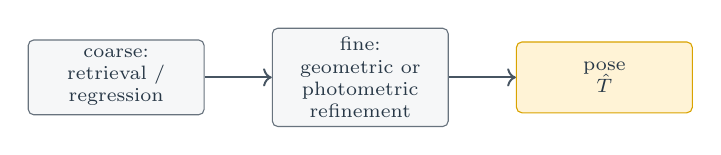
\begin{tikzpicture}[font=\scriptsize\color{ink},
          st/.style={draw=ink!70, fill=ink!4, rounded corners=2pt,
                     align=center, minimum height=9mm, text width=20mm},
          ar/.style={->, line width=0.7pt, draw=ink!85}]
        \node[st] (a) at (0,0) {coarse:\\retrieval / regression};
        \node[st] (b) at (3.1,0) {fine:\\geometric or photometric refinement};
        \node[st, fill=outBg, draw=outLn] (c) at (6.2,0) {pose\\$\hat{T}$};
        \draw[ar] (a) -- (b); \draw[ar] (b) -- (c);
      \end{tikzpicture}
      \end{center}
      \vspace{1mm}
      \begin{itemize}
        \item coarse: rough pose from place recognition or a learned
              regressor;
        \item fine: align the image against the map (features or
              render-and-compare).
      \end{itemize}
      \srcnote{\method{} keeps this recipe --- and threads uncertainty
      through both stages.}
    \end{column}
  \end{columns}
\end{frame}

%--------------------------------------------------------------- 3dgs 101 --
\begin{frame}{From point clouds to Gaussian splatting}
  \begin{columns}[T]
    \begin{column}{0.46\textwidth}
      \textbf{Three generations of maps}
      \begin{itemize}
        \item \textbf{SfM point clouds} ('00s--): sparse 3D points +
              descriptors; match-and-PnP.
        \item \textbf{NeRF} (2020): implicit radiance field;
              photorealistic novel views, but \bad{seconds per frame}.
        \item \textbf{3D Gaussian Splatting} (2023): \emph{explicit}
              anisotropic Gaussians; photorealistic \good{at real-time
              rates}, differentiable.
      \end{itemize}
      \vspace{1mm}
      Each splat: position $\bm\mu$, shape $\bm\Sigma$, opacity, color ---
      and, in semantic variants, a language feature.
    \end{column}
    \begin{column}{0.52\textwidth}
      \textbf{Rendering = sorted alpha-blending}
      \begin{equation*}
        C(\mathbf{x}) \;=\; \sum_i c_i\, \alpha_i(\mathbf{x})
        \prod_{j<i} \big(1 - \alpha_j(\mathbf{x})\big)
      \end{equation*}
      \begin{itemize}
        \item project each Gaussian to the image, composite front-to-back;
        \item fully differentiable w.r.t.\ the camera pose
              $\Rightarrow$ \good{gradient-based pose refinement};
        \item any per-splat quantity can ride along as an extra
              ``color channel.''
      \end{itemize}
      \begin{block}{Remember this equation}
        Later we will blend something unusual through it --- not color,
        but \alert{how much the map trusts itself} at every pixel.
      \end{block}
    \end{column}
  \end{columns}
\end{frame}

%------------------------------------------------------------ uncertainty 101 --
\begin{frame}{Uncertainty 101: two kinds, one test}
  \begin{columns}[T]
    \begin{column}{0.52\textwidth}
      \textbf{Two kinds of not-knowing}
      \begin{itemize}
        \item \textbf{Aleatoric} --- noise in the world: sensor noise,
              motion blur, textureless walls. \emph{Irreducible.}
        \item \textbf{Epistemic} --- gaps in knowledge: unseen viewpoint,
              too little data, \alert{a scene that changed after mapping}.
              \emph{Reducible --- if you know where it is.}
      \end{itemize}
      \vspace{1mm}
      \textbf{One test: calibration.}
      A forecaster who says ``70\% rain'' should be wet on 70\% of those
      days. For poses: a 95\% credible region should contain the true pose
      \textbf{95\% of the time} --- no more (wasteful), no less
      (\bad{dangerous}).
      \vspace{1mm}
      \srcnote{Deep networks are systematically overconfident out of the box
      (Guo et al., ICML 2017) --- softmax scores are not probabilities of
      being right.}
    \end{column}
    \begin{column}{0.45\textwidth}
      \centering
      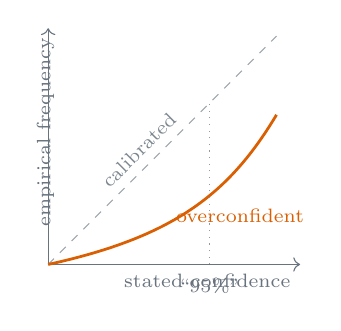
\begin{tikzpicture}[font=\scriptsize\color{ink}]
        \draw[->, ink!70] (0,0) -- (3.2,0) node[below left]{stated confidence};
        \draw[->, ink!70] (0,0) -- (0,3.0) node[rotate=90, above left, yshift=-2mm]{empirical frequency};
        \draw[ink!45, dashed] (0,0) -- (2.9,2.9);
        \node[ink!60, rotate=45] at (1.15,1.45) {calibrated};
        \draw[line width=1pt, uHigh]
          (0,0) .. controls (1.6,0.35) and (2.3,0.9) .. (2.9,1.9);
        \node[uHigh, anchor=west] at (1.5,0.62) {overconfident};
        \draw[ink!50, dotted] (2.05,0) -- (2.05,2.05);
        \node[anchor=north, ink!70] at (2.05,-0.05) {``95\%''};
      \end{tikzpicture}
      \\[2mm]
      \small Below the diagonal: the model promises more than it delivers
      --- the failure mode a safety filter cannot detect from the inside.
    \end{column}
  \end{columns}
\end{frame}

%------------------------------------------------------------------ edl 101 --
\begin{frame}{Evidential deep learning in three minutes}
  \begin{columns}[T]
    \begin{column}{0.52\textwidth}
      \textbf{The softmax prison.} Class probabilities must sum to 1 ---
      there is \bad{no way to say ``I have no idea''}: total ignorance and
      a coin-flip between two classes look identical.
      \vspace{1mm}

      \textbf{The evidential move} (subjective logic): predict non-negative
      \emph{evidence} $e_c$ per class; form an \emph{opinion}
      \begin{equation*}
        b_c = \frac{e_c}{S}, \qquad
        \alert{u = \frac{C}{S}}, \qquad
        S = \textstyle\sum_c (e_c + 1),
      \end{equation*}
      with $\sum_c b_c + u = 1$: belief masses \emph{plus an explicit
      ``I don't know'' mass} --- the \textbf{vacuity}.
      \vspace{1mm}
      \begin{itemize}
        \item Little evidence $\Rightarrow$ $u \to 1$; mountains of
              consistent evidence $\Rightarrow$ $u \to 0$.
        \item Equivalently: a Dirichlet \emph{distribution over the
              softmax} --- uncertainty about the probabilities themselves.
      \end{itemize}
    \end{column}
    \begin{column}{0.45\textwidth}
      \centering
      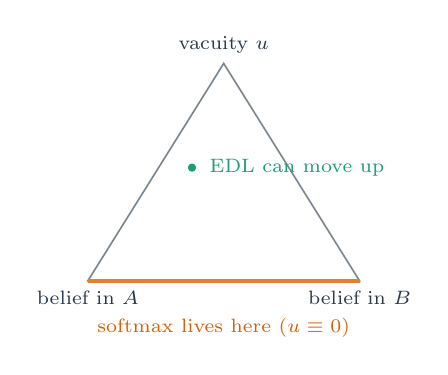
\begin{tikzpicture}[font=\scriptsize\color{ink}, scale=1.15]
        % opinion simplex (2 classes + uncertainty)
        \coordinate (A) at (0,0);
        \coordinate (B) at (3,0);
        \coordinate (U) at (1.5,2.4);
        \draw[ink!60, line width=0.6pt] (A) -- (B) -- (U) -- cycle;
        \node[anchor=north] at (A) {belief in $A$};
        \node[anchor=north] at (B) {belief in $B$};
        \node[anchor=south] at (U) {\alert{vacuity $u$}};
        \draw[line width=1.4pt, uHigh!80] (A) -- (B);
        \node[uHigh, anchor=north, yshift=-3.5mm] at (1.5,0)
          {softmax lives here ($u \equiv 0$)};
        \fill[uLow] (1.15,1.25) circle (1.3pt);
        \node[uLow, anchor=west, xshift=1mm] at (1.15,1.25)
          {EDL can move up};
      \end{tikzpicture}
      \\[2mm]
      \small One extra dimension --- and suddenly ``never seen this'' and
      ``seen it, it's ambiguous'' become \emph{different} outputs.
    \end{column}
  \end{columns}
\end{frame}

%------------------------------------------------------------------ dst 101 --
\begin{frame}{Dempster--Shafer fusion in three minutes}
  \textbf{The question}: two sources give evidential opinions about the same
  thing --- how to combine them?
  \vspace{1mm}
  \begin{columns}[T]
    \begin{column}{0.52\textwidth}
      \textbf{Dempster's rule}: agreement multiplies belief; each side's
      vacuity lets the other side speak.
      \vspace{1mm}
      \begin{center}
      \small
      \begin{tabular}{lcc}
        \toprule
        & belief(chair) & vacuity $u$\\
        \midrule
        sensor A & 0.80 & 0.20\\
        sensor B & 0.70 & 0.30\\
        \midrule
        fused    & \good{0.94} & \good{0.06}\\
        \bottomrule
      \end{tabular}
      \end{center}
      \vspace{1mm}
      Agreement $\Rightarrow$ confidence grows, vacuity shrinks ---
      exactly the behaviour you want when fusing many views of a stable
      object.
    \end{column}
    \begin{column}{0.45\textwidth}
      \begin{block}{Cliffhanger}
        What if the two sources \emph{confidently disagree} --- sensor A
        says ``chair,'' sensor B says ``box''?\\[1mm]
        Intuition: the fused opinion should say \emph{``something is off
        here''} (high vacuity).\\[1mm]
        Dempster's rule says: \bad{confident compromise} --- a famous
        pathology (Zadeh's paradox), and it will come back as a
        \alert{real bug} in the second half of this talk.
      \end{block}
      \vspace{1mm}
      \srcnote{Why care in robotics: ``confident disagreement across
      views'' is the statistical signature of a \emph{moved object}.}
    \end{column}
  \end{columns}
\end{frame}

%==============================================================================
\section{The Problem: Localization Without Honesty}
%==============================================================================

%------------------------------------------------------------ motivation I --
\begin{frame}{Motivation I: the scenario}
  \begin{columns}[T]
    \begin{column}{0.55\textwidth}
      \textbf{An MAV relocalizing in a lived-in room.}
      \begin{itemize}
        \item Pre-built map: photorealistic semantic 3DGS, trained once.
        \item Between mapping and flight, the room \alert{changed}: chairs
              moved, a box appeared, a door opened.
        \item The visual pose is one \emph{measurement} among many --- it is
              injected into a recursive Bayesian estimator (EKF/UKF) and
              fused with IMU and other cues.
      \end{itemize}
      \vspace{1mm}
      \begin{block}{The question the filter actually asks}
        Not ``where am I?'' but
        ``where am I, \textbf{and how much should I believe it}?''
      \end{block}
    \end{column}
    \begin{column}{0.43\textwidth}
      \centering
      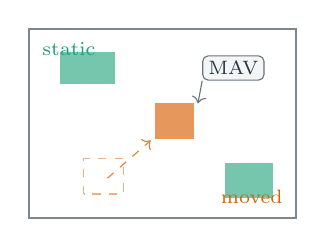
\begin{tikzpicture}[font=\scriptsize\color{ink}]
        % room sketch: static walls + moved objects
        \draw[ink!60, line width=0.7pt] (0,0) rectangle (3.4,2.4);
        \fill[uLow!60]  (0.4,1.7) rectangle (1.1,2.1);   % static shelf
        \fill[uLow!60]  (2.5,0.25) rectangle (3.1,0.7);  % static desk
        \fill[uHigh!65] (1.6,1.0) rectangle (2.1,1.45);  % moved chair
        \draw[uHigh!80, dashed, ->] (1.0,0.5) -- (1.55,0.98);
        \draw[uHigh!50, dashed] (0.7,0.3) rectangle (1.2,0.75); % old position
        \node[anchor=north west] at (0.05,2.35) {\good{static}};
        \node[anchor=south east] at (3.35,0.05) {\bad{moved}};
        % MAV
        \node[draw=ink!70, fill=ink!5, rounded corners=2pt, inner sep=2pt]
          (mav) at (2.6,1.9) {MAV};
        \draw[->, ink!70] (mav.south west) -- (2.15,1.45);
      \end{tikzpicture}
      \\[2mm]
      \small The regions that mislead localization are exactly the ones that
      changed --- and the map could \emph{know} that.
    \end{column}
  \end{columns}
\end{frame}

%----------------------------------------------------------- motivation II --
\begin{frame}{Motivation II: what goes wrong without uncertainty}
  \begin{columns}[T]
    \begin{column}{0.55\textwidth}
      \textbf{A pose without a covariance forces the filter to guess.}
      \begin{itemize}
        \item Fixed measurement noise $\Rightarrow$ \bad{overconfident
              fusion} precisely when the scene is ambiguous, occluded,
              changed, or texture-poor.
        \item Hard robust-object masks (LLM-selected) are \bad{discrete}:
              an object is either trusted or discarded --- and the selector
              itself has documented failure cases.
        \item Retrieval ambiguity makes the error
              \bad{multi-modal} --- a single Gaussian, let alone a point,
              cannot represent ``it is here \emph{or} there.''
      \end{itemize}
    \end{column}
    \begin{column}{0.43\textwidth}
      \begin{block}{Requirements for the output}
        \small
        \begin{enumerate}
          \item[R1] \textbf{Calibrated}: credibility-$\alpha$ regions
                contain the truth with frequency $\alpha$.
          \item[R2] \textbf{Graded}: trust in map content is continuous,
                not a binary mask.
          \item[R3] \textbf{Multi-modal}: ambiguity survives to the output
                as a mixture, not averaged away.
        \end{enumerate}
      \end{block}
      \vspace{1mm}
      \small \method{} is designed backwards from R1--R3.
    \end{column}
  \end{columns}
\end{frame}

%==============================================================================
\section{Related Work: Four Families, One Shared Blind Spot}
%==============================================================================

%--------------------------------------------------------- related work I --
\begin{frame}{Related work I: visual localization --- strengths \& limitations}
  \centering
  \scriptsize
  \renewcommand{\arraystretch}{1.35}
  \begin{tabular}{@{}p{21mm}p{34mm}p{33mm}>{\color{uHigh}}p{46mm}@{}}
    \toprule
    \normalfont\textbf{Family} & \textbf{Representatives} &
    \textbf{Strength} & \textbf{\color{ink}Limitation}\\
    \midrule
    Absolute pose regression &
    PoseNet (ICCV'15), MS-Transf.\ (ICCV'21), Marepo (CVPR'24) &
    fast, storage-light, end-to-end &
    accuracy tied to training views; no geometric reasoning; silently
    overconfident off-distribution\\
    Scene coordinate regression &
    DSAC* (TPAMI'21), ACE (CVPR'23), GLACE, ACE0 (ECCV'24) &
    the scene-specific accuracy reference &
    per-scene training; degrades in clutter and repetitive layouts;
    ACE-G's coordinate uncertainty is consumed internally\\
    Feature matching \& feed-forward &
    SuperGlue/LightGlue; MASt3R (ECCV'24), Reloc3r (CVPR'25) &
    scene-agnostic, strong generalization &
    low-level features sensitive to lighting/texture; per-correspondence
    confidences never leave the pipeline\\
    Semantic localization &
    CLIP-Loc (ICRA'24), SceneGraphLoc (ECCV'24) &
    robust association at object / scene-graph level &
    coarse: no metric 6-DoF pose distribution; semantics as labels, not
    as evidence\\
    \bottomrule
  \end{tabular}
  \vspace{2mm}
  \begin{block}{The shared blind spot}
    Uncertainty, where it exists at all, is an \emph{internal ingredient}
    --- \alert{none of these reports a calibrated pose covariance}.
  \end{block}
\end{frame}

%-------------------------------------------------------- related work II --
\begin{frame}{Related work II: rendering-based localization --- strengths \& limitations}
  \centering
  \scriptsize
  \renewcommand{\arraystretch}{1.35}
  \begin{tabular}{@{}p{20mm}p{36mm}p{31mm}>{\color{uHigh}}p{47mm}@{}}
    \toprule
    \normalfont\textbf{Family} & \textbf{Representatives} &
    \textbf{Strength} & \textbf{\color{ink}Limitation}\\
    \midrule
    NeRF refiners &
    iNeRF (IROS'21), NeFeS, CrossFire (ICCV'23), NeRFMatch (ECCV'24) &
    photometrically precise render-and-compare &
    slow rendering; lighting-sensitive; point output\\
    Particle beliefs &
    Loc-NeRF (ICRA'23), MCLoc (CVPR'24) &
    global search; maintains a genuine pose belief &
    hundreds of renders per query; belief is uncalibrated and then
    discarded --- only its MAP is reported\\
    3DGS wave &
    iComMa, GS-CPR (ICLR'25), GSplatLoc (IROS'25), HGSLoc/LoGS (ICRA'25),
    STDLoc/GSFFs (CVPR'25), SplatHLoc (CVPR'26) &
    real-time rendering; sub-cm accuracy &
    uniformly point outputs; static-scene assumption; no notion of map
    trustworthiness\\
    Uncertainty-guided &
    UGS-Loc (CVPR'26) &
    Fisher-information maps guide particles + RANSAC $\Rightarrow$
    best accuracy &
    uncertainty is post-hoc, purely geometric, and internal: no
    covariance, no calibration, no semantics\\
    Semantic 3DGS &
    SGLoc (IROS'25), Chu \& Kim (RA-L'26) &
    robustness to scene change via semantics &
    SGLoc: no uncertainty, refinement coupled to own retrieval;
    Chu \& Kim: discrete LLM object gating with documented failures\\
    \bottomrule
  \end{tabular}
  \vspace{1.5mm}
  \begin{block}{The shared blind spot}
    The belief either never exists, is used \emph{internally}, or dies
    before the output --- \alert{no rendering-based localizer emits a
    calibrated pose distribution}.
  \end{block}
\end{frame}

%------------------------------------------------------- related work III --
\begin{frame}{Related work III: uncertainty methods --- strengths \& limitations}
  \centering
  \scriptsize
  \renewcommand{\arraystretch}{1.35}
  \begin{tabular}{@{}p{22mm}p{34mm}p{30mm}>{\color{uHigh}}p{48mm}@{}}
    \toprule
    \normalfont\textbf{Family} & \textbf{Representatives} &
    \textbf{Strength} & \textbf{\color{ink}Limitation}\\
    \midrule
    Bayesian / variational APR &
    Bayesian PoseNet (ICRA'16), VaPoR (ICRA'23) &
    genuine distribution outputs &
    inherits APR's accuracy ceiling; static scenes; uncalibrated\\
    Scalar gates &
    HR-APR (ICRA'24) &
    cheap; APR-agnostic &
    one number used only to gate refinement --- not a distribution\\
    Probabilistic PnP \& conformal &
    EPro-PnP (CVPR'22), PURSE (CVPR'23) &
    principled $SE(3)$ densities / statistical guarantees &
    object-centric or map-free --- no scene-scale relocalization\\
    Distributional error models &
    Wu \& Campbell (ICRA'25) &
    shows pose error is non-Gaussian $\Rightarrow$ GMM &
    2D image retrieval only --- no 3D map, no rendering; we lift it to
    6-DoF\\
    Evidential localization &
    Chen et al.\ (ICRA'24), SCREP &
    EDL reaches scene-coordinate regression &
    no metric map at query time; uncertainty not propagated to a
    calibrated posterior\\
    Uncertainty-aware mapping &
    S-BKI/ConvBKI; EBS (IROS'24), E$^2$-BKI (RA-L'26), CSS (ICRA'25),
    PhysGS (CVPR'26); FisherRF, Bayes' Rays; WildGS-SLAM &
    trustworthy maps; per-primitive beliefs &
    never localizes a query --- uncertainty stays inside the map or the
    tracking loss\\
    \bottomrule
  \end{tabular}
  \vspace{1.5mm}
  \begin{columns}[T]
    \begin{column}{0.99\textwidth}
      \begin{block}{The shared blind spot}
        Rigorous uncertainty exists on \emph{both} sides ---
        \alert{but it never travels from the map to the pose the robot
        consumes}. \method{}'s job is exactly that transport.
      \end{block}
    \end{column}
  \end{columns}
  \vspace{1mm}
  \srcnote{We transplant the evidential machinery from mapping (scoring
  observations) to localization (scoring correspondences and pixels).}
\end{frame}

%---------------------------------------------------------------------- gap --
\begin{frame}{The open cell in the design space}
  \begin{columns}[T]
    \begin{column}{0.52\textwidth}
      \centering
      \resizebox{\linewidth}{!}{\input{\figpath fig2_positioning}}
    \end{column}
    \begin{column}{0.46\textwidth}
      \small
      \textbf{Closest neighbours (2023--2026):}
      \begin{itemize}
        \item \textbf{UGS-Loc} (CVPR'26): Fisher-information uncertainty
              \emph{inside} a 3DGS refiner --- consumed internally,
              \bad{point output}.
        \item Particle localizers (Loc-NeRF, MCLoc): keep a belief,
              \bad{report only its MAP, uncalibrated}.
        \item E$^2$-BKI, EBS, CSS: evidential \emph{maps},
              \bad{no query localization}.
        \item Wu \& Campbell (ICRA'25): error distribution, \bad{2D retrieval
              only}.
      \end{itemize}
      \vspace{1mm}
      \begin{block}{\method{} claim}
        First localizer to output a \textbf{calibrated $SE(3)$ pose
        distribution} from a Gaussian-splatting map, with evidential
        semantics propagated end-to-end.
      \end{block}
    \end{column}
  \end{columns}
\end{frame}

%==============================================================================
\section{\method{}: Carrying Uncertainty from Map to Pose}
%==============================================================================

%------------------------------------------------------------------ key idea --
\begin{frame}{Key idea: one uncertainty channel, carried end-to-end}
  \textbf{Vacuity} $u$ --- the evidential ``I don't know'' mass --- is born at
  the observation, fused into the map, and \emph{never dropped}: every stage
  consumes it in its own natural form.
  \vspace{2mm}
  \begin{center}
  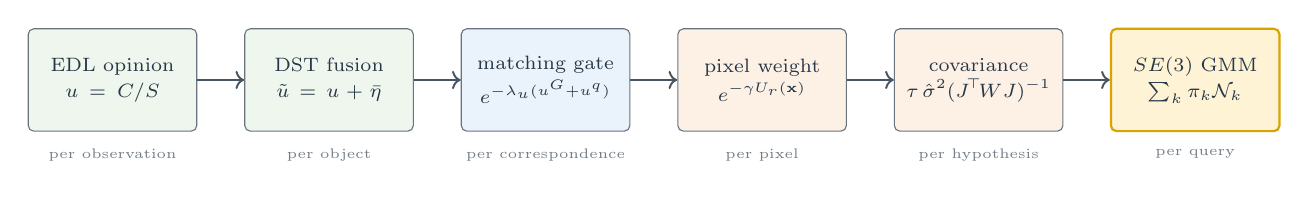
\begin{tikzpicture}[
      font=\scriptsize\color{ink},
      st/.style={draw=ink!70, fill=white, rounded corners=2pt, align=center,
                 minimum height=13mm, text width=20mm, inner sep=2pt},
      lab/.style={font=\tiny\color{ink!65}, align=center},
      ar/.style={->, line width=0.7pt, draw=ink!85}]
    \node[st, fill=encBg]    (s1) at (0,0)    {EDL opinion\\[0.5mm]$u = C/S$};
    \node[st, fill=encBg]    (s2) at (2.75,0) {DST fusion\\[0.5mm]$\tilde{u} = u + \bar\eta$};
    \node[st, fill=coarseBg] (s3) at (5.5,0)  {matching gate\\[0.5mm]$e^{-\lambda_u(u^G+u^q)}$};
    \node[st, fill=fineBg]   (s4) at (8.25,0) {pixel weight\\[0.5mm]$e^{-\gamma U_r(\mathbf{x})}$};
    \node[st, fill=fineBg]   (s5) at (11.0,0) {covariance\\[0.5mm]$\tau\,\hat\sigma^2 (J^{\!\top}\! W J)^{-1}$};
    \node[st, fill=outBg, draw=outLn, line width=0.8pt] (s6) at (13.75,0)
      {$SE(3)$ GMM\\[0.5mm]$\sum_k \pi_k \mathcal{N}_k$};
    \draw[ar] (s1) -- (s2); \draw[ar] (s2) -- (s3);
    \draw[ar] (s3) -- (s4); \draw[ar] (s4) -- (s5); \draw[ar] (s5) -- (s6);
    \node[lab, below=1mm of s1] {per observation};
    \node[lab, below=1mm of s2] {per object};
    \node[lab, below=1mm of s3] {per correspondence};
    \node[lab, below=1mm of s4] {per pixel};
    \node[lab, below=1mm of s5] {per hypothesis};
    \node[lab, below=1mm of s6] {per query};
  \end{tikzpicture}
  \end{center}
  \vspace{2mm}
  \begin{itemize}
    \item No hand-tuned dynamic-object heuristics, no LLM in the loop:
          the map's \emph{own} uncertainty does the gating.
    \item Query and map share \textbf{the same evidential head}, so their
          vacuities are directly comparable.
  \end{itemize}
\end{frame}

%-------------------------------------------------------------- contributions --
\begin{frame}{Contributions}
  \begin{enumerate}
    \item \textbf{A calibrated-distribution localizer on a 3DGS map.}
          Evidential (EDL + Dempster--Shafer) semantic uncertainty is
          integrated end-to-end from map construction to the pose output ---
          prior 3DGS localizers ignore uncertainty, use it internally
          (UGS-Loc), or keep uncalibrated beliefs (particle filters,
          GS-SLAM).
    \vspace{1mm}
    \item \textbf{Uncertainty-weighted 2D--3D semantic matching.}
          Correspondences gated by evidential vacuity; ambiguous retrieval
          yields a \emph{weighted pose mixture} --- lifting the
          non-Gaussian-error insight of Wu \& Campbell from 2D retrieval to
          6-DoF.
    \vspace{1mm}
    \item \textbf{Uncertainty-aware differentiable-rendering refinement.}
          Per-pixel weights from alpha-blended primitive vacuity --- a graded
          replacement for discrete robust-object masks --- plus a Laplace
          pose covariance at the optimum, tempered on a held-out split.
    \vspace{1mm}
    \item \textbf{A calibration-centric evaluation protocol.}
          Coverage vs.\ $\chi^2$, AUSE, NLL, ECE on standard and
          semi-dynamic indoor benchmarks --- metrics essentially absent
          from prior localization work.
  \end{enumerate}
\end{frame}

%------------------------------------------------------------------ overview --
\begin{frame}{\method{} at a glance}
  \centering
  \resizebox{\textwidth}{!}{\input{\figpath fig1_overview}}
  \vspace{3mm}
  \begin{itemize}\small
    \item \textbf{Coarse}: evidential instances $\rightarrow$ vacuity-gated
          retrieval $\rightarrow$ top-$k$ pose hypotheses with weights.
    \item \textbf{Fine}: each hypothesis refined by vacuity-weighted
          differentiable rendering; covariance from the loss curvature.
    \item \textbf{Output}: pruned, weighted $SE(3)$ Gaussian mixture;
          condensed to one Gaussian for the filter.
  \end{itemize}
\end{frame}

%------------------------------------------------------- problem formulation --
\begin{frame}{Problem formulation}
  \textbf{Given} a pre-built semantic Gaussian map
  $\mathcal{M} = \{\mathcal{G}_i\}_{i=1}^{M}$ and a query image $I_q$,
  estimate the \textbf{full posterior} --- not
  $\hat{T} = \arg\max_T s(I_q, T; \mathcal{M})$:
  \begin{equation*}
    p\big(T \mid I_q, \mathcal{M}\big), \qquad T \in SE(3),
  \end{equation*}
  \textbf{subject to calibration}: a credibility-$\alpha$ region of the
  posterior contains the ground-truth pose with empirical frequency
  $\alpha$.
  \vspace{2mm}
  \begin{columns}[T]
    \begin{column}{0.5\textwidth}
      \begin{block}{Reference primitive (map side)}
        \small
        $\mathcal{G}_i = (\bm\mu_i,\ \bm\Sigma_i,\ f_i,\ \mathbf{p}_i,\ u_i)$\\[1mm]
        3D mean, covariance (anisotropic geometry), CLIP embedding,
        semantic probability, \alert{vacuity mass $u_i \in [0,1]$}.
      \end{block}
    \end{column}
    \begin{column}{0.5\textwidth}
      \begin{block}{Query instance (image side)}
        \small
        $\mathcal{Q}_j = (\mathbf{x}_j,\ a_j,\ f_j^q,\ \mathbf{p}_j^q,\ u_j^q)$\\[1mm]
        2D centroid, area, and the \emph{same} semantic triplet ---
        both sides live in one evidential space.
      \end{block}
    \end{column}
  \end{columns}
  \vspace{2mm}
  \small Uncertainty is \emph{first-class on both sides} before any matching
  happens --- that is what makes end-to-end propagation possible.
\end{frame}

%------------------------------------------------- method 1a: EDL opinions --
\begin{frame}{Method 1a: evidential opinions from a shared head}
  \begin{columns}[T]
    \begin{column}{0.55\textwidth}
      \textbf{Evidential Deep Learning (EDL).} A segmentation head outputs
      non-negative \emph{evidence} $e = [e_1, \dots, e_C]$, interpreted as a
      Dirichlet with $\alpha_c = e_c + 1$, $S = \sum_c \alpha_c$:
      \begin{equation*}
        \hat{p}_c = \frac{\alpha_c}{S}, \qquad
        b_c = \frac{\alpha_c - 1}{S}, \qquad
        \alert{u = \frac{C}{S}},
      \end{equation*}
      with $u + \sum_c b_c = 1$.
      \begin{itemize}
        \item Little total evidence $S$ $\Rightarrow$ large vacuity $u$:
              the network \emph{saying} it does not know.
        \item Trained with the EDL loss: Dirichlet Brier risk + KL that
              drives misleading evidence toward the uniform prior.
      \end{itemize}
    \end{column}
    \begin{column}{0.43\textwidth}
      \begin{block}{One head, two consumers}
        \small The \emph{same} evidential head encodes
        \begin{itemize}
          \item map-building observations (distilled into splats), and
          \item Fast-SAM + CLIP query instances at test time,
        \end{itemize}
        so $u^G$ and $u^q$ are on the same scale --- required for the
        matching gate later.
      \end{block}
      \vspace{2mm}
      \small Contrast with softmax: probabilities always sum to 1 and
      \emph{cannot} express ``no evidence at all'' --- the ablation
      (EDL vs.\ softmax) isolates exactly this.
    \end{column}
  \end{columns}
\end{frame}

%---------------------------------------------- method 1b: map construction --
\begin{frame}{Method 1b: from splats to evidential primitives}
  \begin{columns}[T]
    \begin{column}{0.55\textwidth}
      \textbf{Object-level clustering} (Gaussian-Grouping-style identity
      features), then per cluster $\mathcal{C}_i$:
      \begin{itemize}
        \item geometry: empirical $\bm\mu_i, \bm\Sigma_i$ of member centroids;
        \item CLIP feature $f_i$: \emph{vacuity-weighted} average ---
              confident members dominate;
        \item semantics: \textbf{Dempster fusion} of member opinions
      \end{itemize}
      \begin{equation*}
        b^c = \tfrac{1}{1-\eta}\!\left(b_1^c b_2^c + b_1^c u_2 + b_2^c u_1\right),
        \quad u = \tfrac{u_1 u_2}{1-\eta},
      \end{equation*}
      where $\eta = \sum_{x \neq y} b_1^x b_2^y$ measures conflict.
    \end{column}
    \begin{column}{0.43\textwidth}
      \begin{block}{\alert{Caveat we hit in practice (Zadeh)}}
        \small Dempster's rule \emph{renormalizes conflict away}: two
        confident, contradictory opinions (a moved object!) fuse to
        \bad{low} vacuity --- the opposite of what we need.\\[1mm]
        Fix: accumulate $\bar\eta_i$ and use the \textbf{effective vacuity}
        $\tilde{u}_i = \min(1,\, u_i + \bar\eta_i)$ (equivalently Yager's
        rule). Numeric example in backup.
      \end{block}
      \vspace{1mm}
      \centering
      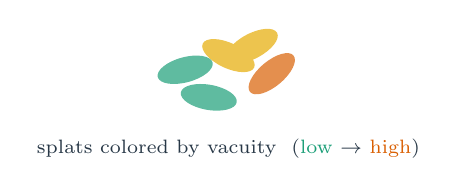
\begin{tikzpicture}[font=\scriptsize\color{ink}]
        \foreach \x/\y/\a/\c in {0/0/15/uLow, 0.55/0.18/-25/uMid, 1.1/-0.05/40/uHigh,
                                 0.3/-0.35/-10/uLow, 0.85/0.3/28/uMid}{
          \fill[\c!70, rotate around={\a:(\x,\y)}] (\x,\y) ellipse (3.6mm and 1.6mm);
        }
        \node[below=4mm, anchor=north] at (0.55,-0.35)
          {splats colored by vacuity \ (\good{low} $\to$ \bad{high})};
      \end{tikzpicture}
    \end{column}
  \end{columns}
\end{frame}

%------------------------------------------- method 2: encoding + matching --
\begin{frame}{Method 2: evidential query encoding \& gated matching}
  \textbf{Instance descriptors in a shared space.} Fast-SAM masks
  $\rightarrow$ CLIP + EDL per instance; geometry enters through small MLPs:
  \begin{equation*}
    d_j^q = \mathrm{MLP}\big[\,\phi(f_j^q) \,\|\, \psi_{\mathbf{x}}(\mathbf{x}_j)
    \,\|\, \psi_a(a_j)\,\big],
    \qquad
    d_i^G \text{ analogously from } (f_i, \bm\mu_i, \bm\Sigma_i)
    \text{ in the camera frame.}
  \end{equation*}
  \begin{columns}[T]
    \begin{column}{0.52\textwidth}
      \begin{block}{Gated instance similarity}
        \begin{equation*}
          s_{ij} =
          \underbrace{\cos\!\big(d_i^G, d_j^q\big)}_{\text{semantic similarity}}
          \cdot
          \underbrace{e^{-\lambda_u (u_i^G + u_j^q)}}_{\text{evidential gate}}
        \end{equation*}
      \end{block}
      \small Confident--confident pairs dominate; moved or ambiguous
      instances contribute weakly --- on \emph{either} side.
    \end{column}
    \begin{column}{0.46\textwidth}
      \textbf{Scene-level retrieval} (SGLoc-style):
      \begin{itemize}\small
        \item self-attention + gated attention pooling
              $\rightarrow$ scene descriptor per submap / query;
        \item trained with symmetric InfoNCE (2D $\leftrightarrow$ 3D)
              + EDL loss for the heads;
        \item top-$k$ submaps $\Rightarrow$ hypotheses
              $\{(T_0^k, \tilde\pi_k)\}$ --- ambiguity becomes an explicit
              \alert{pose mixture}.
      \end{itemize}
    \end{column}
  \end{columns}
\end{frame}

%------------------------------------------------ method 3: refinement -----
\begin{frame}{Method 3: uncertainty-aware rendering refinement}
  \begin{columns}[T]
    \begin{column}{0.56\textwidth}
      \textbf{Vacuity rendered like color} (same alpha-blending kernel,
      one extra channel):
      \begin{equation*}
        U_r(\mathbf{x}) = \sum_i u_i\, \alpha_i(\mathbf{x})
        \prod_{j<i}\big(1 - \alpha_j(\mathbf{x})\big)
      \end{equation*}
      \textbf{Weighted objective} in the tangent space,
      $T(\bm\xi) = \exp(\bm\xi^\wedge)\, T_0$:
      \begin{equation*}
        E(\bm\xi) = \sum_{\mathbf{x}}
        \alert{w(\mathbf{x})}\,\big\|I_q(\mathbf{x}) - I_r(\mathbf{x};\bm\xi)\big\|^2
        + \lambda \sum_k \|\mathbf{x}_k^q - \mathbf{x}_k^r\|^2
      \end{equation*}
      with $w(\mathbf{x}) = \exp(-\gamma\, U_r(\mathbf{x}))$; sparse
      keypoint term optional.
    \end{column}
    \begin{column}{0.42\textwidth}
      \begin{itemize}
        \item Moved objects, texture-poor and semantically uncertain regions
              are down-weighted \emph{continuously} --- the graded
              replacement for hard robust-object masks (R2).
        \item Weights \textbf{detached per iterate} (IRLS-style): otherwise
              the optimizer ``hides'' misalignment in high-vacuity regions
              instead of fixing the pose (backup slide).
        \item Training-free; plugs into any differentiable rasterizer.
      \end{itemize}
    \end{column}
  \end{columns}
\end{frame}

%---------------------------------------------- method 4: covariance -------
\begin{frame}{Method 4: from optimum to covariance --- Laplace + temperature}
  \begin{columns}[T]
    \begin{column}{0.55\textwidth}
      \textbf{Laplace approximation} at the optimum $\bm\xi^\star$, with
      stacked weighted residuals $\mathbf{r}$ and Jacobian
      $J = \partial\mathbf{r}/\partial\bm\xi|_{\bm\xi^\star}$:
      \begin{equation*}
        \bm\xi \sim \mathcal{N}\big(\bm\xi^\star,\ \bm\Sigma_{\bm\xi}\big),
        \qquad
        \bm\Sigma_{\bm\xi} \approx \hat\sigma^2 \big(J^\top W J\big)^{-1}
      \end{equation*}
      \begin{itemize}
        \item Flat photometric basin (weak constraint) $\Rightarrow$ large
              covariance; sharp basin $\Rightarrow$ tight one.
        \item $\hat\sigma^2$ from the residuals: degraded queries
              \emph{automatically} get larger covariances.
        \item Reuses the refinement machinery --- negligible overhead.
      \end{itemize}
    \end{column}
    \begin{column}{0.43\textwidth}
      \begin{block}{Honesty requires tempering}
        \small Real photometric residuals are heavy-tailed and spatially
        correlated $\Rightarrow$ raw Laplace is \bad{overconfident}. A
        single scalar $\tau$ fitted on a held-out split,
        \begin{equation*}
          \bm\Sigma \leftarrow \tau \bm\Sigma, \qquad
          \tau = \mathrm{med}(d^2)\,/\,\chi^2_{6,0.5},
        \end{equation*}
        restores nominal coverage (robust to wrong-basin outliers).
      \end{block}
      \small Synthetic evidence: ECE $0.50 \!\to\! 0.16$ with
      $\tau \approx 27$; AUSE stays low --- \emph{informative} before,
      \emph{honest} after.
    \end{column}
  \end{columns}
\end{frame}

%------------------------------------------------ method 5: output ---------
\begin{frame}{Method 5: the calibrated Gaussian mixture on $SE(3)$}
  \begin{equation*}
    p\big(T \mid I_q, \mathcal{M}\big)
    = \sum_k \pi_k\, \mathcal{N}\!\big(\bm\xi;\ \bm\xi_k^\star,\ \bm\Sigma_{\bm\xi,k}\big),
    \qquad \pi_k \propto \text{retrieval weight} \times \text{render fidelity}
  \end{equation*}
  \begin{columns}[T]
    \begin{column}{0.55\textwidth}
      \begin{itemize}
        \item Fidelity (PSNR) pruning removes hypotheses whose renders
              diverge from $I_q$.
        \item \textbf{Condensation} by moment matching:
              $\bm\mu = \sum_k \pi_k \bm\xi_k^\star$,\quad
              $\bm\Sigma = \sum_k \pi_k\big(\bm\Sigma_k +
              (\bm\xi_k^\star{-}\bm\mu)(\bm\xi_k^\star{-}\bm\mu)^\top\big)$
        \item $\Rightarrow$ a single Gaussian a downstream EKF/UKF consumes
              directly (R1 + R3 reconciled: keep the mixture, hand over the
              summary).
        \item Rotation alternative: Bingham on the quaternion --- ablated.
      \end{itemize}
    \end{column}
    \begin{column}{0.42\textwidth}
      \centering
      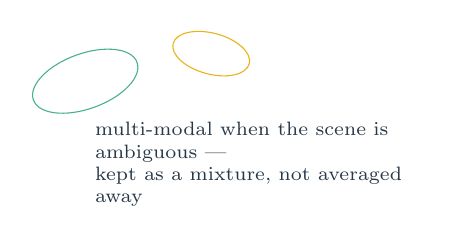
\begin{tikzpicture}[font=\scriptsize\color{ink}]
        \coordinate (a) at (0,0);
        \coordinate (b) at (1.6,0.35);
        \draw[uLow!80, rotate around={20:(a)}]  (a) ellipse (7mm and 3.5mm);
        \draw[uMid!90, rotate around={-15:(b)}] (b) ellipse (5mm and 2.6mm);
        \node[below=4mm of a, anchor=north west, text width=42mm]
          {multi-modal when the scene is ambiguous ---\\
           kept as a mixture, not averaged away};
      \end{tikzpicture}
    \end{column}
  \end{columns}
\end{frame}

%------------------------------------------------------------- algorithm ---
\begin{frame}{Algorithm: one query image}
  \begin{enumerate}
    \item Fast-SAM masks of $I_q$; CLIP + EDL per instance
          $\rightarrow$ evidential query instances $\{\mathcal{Q}_j\}$.
    \item Build instance descriptors $d_j^q$ and the gated scene descriptor
          $F^q$.
    \item Score submaps by gated similarity; take top-$k$ $\rightarrow$
          hypotheses $\{(T_0^k, \tilde\pi_k)\}$.
    \item \textbf{For each hypothesis}: refine by minimizing
          $E(\bm\xi)$ with per-pixel weight $w = e^{-\gamma U_r}$;
          compute $\bm\Sigma_{\bm\xi,k}$ by Laplace; apply temperature
          $\tau$.
    \item Prune by render fidelity; assemble the GMM; condense by moment
          matching.
    \item \textbf{Return} $p(T \mid I_q, \mathcal{M})$ and its
          single-Gaussian summary for the filter.
  \end{enumerate}
  \vspace{2mm}
  \srcnote{Steps 1--3: coarse stage (learned, trained with InfoNCE + EDL
  loss). Steps 4--6: fine stage (training-free). The temperature $\tau$ is
  fitted once per scene on a held-out calibration split.}
\end{frame}

%==============================================================================
\section{Evaluation: Making Calibration the Headline}
%==============================================================================

%--------------------------------------------------------------- datasets --
\begin{frame}{Datasets}
  \centering
  \small
  \begin{tabular}{llll}
    \toprule
    Dataset & Content & Ground truth & Role \\
    \midrule
    7Scenes  & 7 rooms, RGB-D Kinect & \alert{SfM pseudo-GT} & accuracy vs.\ SOTA\\
    12Scenes & 12 rooms / 4 environments & dataset RGB-D GT & larger-scale accuracy\\
    ScanNet  & 1{,}513 indoor scans & dataset GT & diversity + calibration\\
    Semi-dynamic & rearranged objects & --- & robustness + honest $\bm\Sigma$ growth\\
    \bottomrule
  \end{tabular}
  \vspace{3mm}
  \begin{columns}[T]
    \begin{column}{0.52\textwidth}
      \begin{block}{Why SfM pseudo-GT on 7Scenes (a real trap)}
        \small The same method differs wildly between DSLAM and SfM
        conventions (ACE: 80.8\% vs.\ 97.1\% @5cm/5$^\circ$). All recent
        3DGS localizers report SfM --- mixing conventions silently is the
        most common citation error in this space.
      \end{block}
    \end{column}
    \begin{column}{0.46\textwidth}
      \textbf{Semi-dynamic protocol} (following Chu \& Kim):
      \begin{itemize}\small
        \item objects rearranged between mapping and query;
        \item high- vs.\ low-quality maps ($\sim$1000 vs.\ $\sim$300
              mapping images);
        \item degraded-semantics stress test: the covariance must
              \emph{grow} as conditions worsen.
      \end{itemize}
    \end{column}
  \end{columns}
\end{frame}

%----------------------------------------------------------------- metrics --
\begin{frame}{Metrics: accuracy \emph{and} calibration}
  \small
  \begin{columns}[T]
    \begin{column}{0.5\textwidth}
      \textbf{Accuracy} (standard)
      \begin{itemize}
        \item median translation / rotation error (cm / $^\circ$);
        \item success rate @ 5cm/5$^\circ$ and 2cm/2$^\circ$.
      \end{itemize}
      \vspace{1mm}
      \textbf{Calibration} (the headline --- each answers one question)
      \begin{itemize}
        \item \textbf{Coverage}: is the covariance honest?\\
              $\Pr\!\big[d^2 \le \chi^2_{6}(\alpha)\big] \overset{?}{=} \alpha$
              at $\alpha = 68.3 / 95.4 / 99.7\%$,\\
              $d^2 = \mathbf{e}^\top \bm\Sigma^{-1} \mathbf{e}$,
              $\mathbf{e} = \log\!\big(T_{gt} T_{est}^{-1}\big)$.
        \item \textbf{ECE}: summary miscalibration ---
              mean $|\text{coverage}(\alpha) - \alpha|$ over a level grid.
        \item \textbf{AUSE}: is uncertainty \emph{informative} per query?
              Area between the sparsification curve (rank by predicted
              $\sigma$) and the oracle (rank by true error).
        \item \textbf{NLL} of the true pose under the GMM: distribution
              quality including multi-modality.
      \end{itemize}
    \end{column}
    \begin{column}{0.46\textwidth}
      \centering
      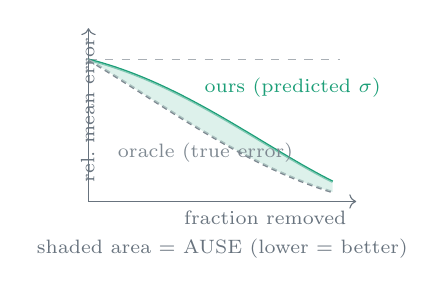
\begin{tikzpicture}[font=\scriptsize\color{ink}, scale=1.0]
        % sparsification sketch
        \draw[->, ink!70] (0,0) -- (3.4,0) node[below left]{fraction removed};
        \draw[->, ink!70] (0,0) -- (0,2.2) node[rotate=90, above left, yshift=-2mm]{rel.\ mean error};
        \draw[ink!40, dashed] (0,1.8) -- (3.2,1.8);
        \draw[line width=0.9pt, uLow]
          (0,1.8) .. controls (1.2,1.5) and (2.2,0.7) .. (3.1,0.25);
        \draw[line width=0.9pt, ink!60, dash pattern=on 2pt off 1.5pt]
          (0,1.8) .. controls (1.0,1.2) and (2.0,0.45) .. (3.1,0.12);
        \fill[uLow!25, opacity=0.6]
          (0,1.8) .. controls (1.2,1.5) and (2.2,0.7) .. (3.1,0.25) --
          (3.1,0.12) .. controls (2.0,0.45) and (1.0,1.2) .. (0,1.8) -- cycle;
        \node[uLow, anchor=west] at (1.35,1.45) {ours (predicted $\sigma$)};
        \node[ink!60, anchor=west] at (0.25,0.62) {oracle (true error)};
        \node[anchor=north, ink!70] at (1.7,-0.35)
          {shaded area $=$ AUSE (lower $=$ better)};
      \end{tikzpicture}
      \vspace{2mm}
      \begin{block}{Why both AUSE and coverage}
        \small A covariance can \emph{rank} errors perfectly (low AUSE) yet
        be 10$\times$ too small (bad coverage) --- and vice versa. Honest
        \emph{and} informative requires both.
      \end{block}
    \end{column}
  \end{columns}
\end{frame}

%------------------------------------------------------------------- sota ---
\begin{frame}{Where the field stands (7Scenes, SfM pseudo-GT, median cm/$^\circ$)}
  \centering
  \begin{tabular}{lccc}
    \toprule
    Method & Venue & Avg.\ error & Pose uncertainty?\\
    \midrule
    ACE / DSAC*        & CVPR'23 / TPAMI'21 & 1.1/0.34 & \bad{none}\\
    GSplatLoc          & IROS'25  & 1.4/0.37 & \bad{none}\\
    GS-CPR (ACE init)  & ICLR'25  & 0.8/0.25 & \bad{none}\\
    STDLoc             & CVPR'25  & 0.8/0.24 & \bad{none}\\
    UGS-Loc (ACE init) & CVPR'26  & 0.6/0.21 & \bad{internal only, point out}\\
    SplatHLoc          & CVPR'26  & 0.6/0.17 & \bad{none}\\
    \textbf{\method{} (ours)} & --- & \res & \good{\textbf{calibrated $SE(3)$ GMM}}\\
    \bottomrule
  \end{tabular}
  \vspace{2mm}\\
  \srcnote{Numbers as reported in the cited papers (see paper Table I for
  per-scene values and sources). SGLoc reports 0.5/0.15 but on 4/7 scenes
  under DSLAM GT --- not comparable.}
  \vspace{2mm}
  \begin{itemize}
    \item Goal: stay competitive with this group while \alert{additionally}
          producing the covariance none of them reports.
    \item Baselines also include APR (PoseNet, Marepo), NeRF-based
          (NeFeS, CrossFire, PNeRFLoc), and the semantic localizers
          SGLoc / Chu \& Kim on their own protocols.
  \end{itemize}
\end{frame}

%------------------------------------------------------- synthetic evidence --
\begin{frame}{Implementation status \& synthetic evidence}
  \textbf{Full pipeline implemented} (PyTorch, 61 unit tests; gsplat or
  pure-torch renderer): EDL/DST fusion, gated retrieval, vacuity-weighted
  refinement, Laplace + temperature, $SE(3)$ GMM, all calibration metrics.
  \vspace{1mm}
  \begin{columns}[T]
    \begin{column}{0.55\textwidth}
      \textbf{Semi-dynamic synthetic benchmark} (25\% of objects moved
      after mapping):
      \begin{itemize}\small
        \item Map vacuity separates content with \emph{no thresholds}:
              dynamic \bad{0.67} vs.\ static \good{0.16}.
        \item Median 5.8\,cm / 0.9$^\circ$; wrong-basin queries appear as
              extra mixture modes (the multi-modality is real).
        \item $K{=}1$ ablation degrades to 8.6\,cm and SR
              37.5\% $\to$ 25\% --- the mixture earns its keep.
      \end{itemize}
    \end{column}
    \begin{column}{0.43\textwidth}
      \centering
      \small
      \begin{tabular}{lcc}
        \toprule
        & ECE $\downarrow$ & AUSE$_t$ $\downarrow$\\
        \midrule
        raw Laplace      & \bad{0.50} & 0.05\\
        + temperature    & \good{0.16} & 0.07\\
        fixed covariance & 0.18 & \bad{0.67}\\
        \bottomrule
      \end{tabular}
      \\[2mm]
      \srcnote{informative (low AUSE) $\ne$ honest (low ECE):\\
      you need both, and only ours has both.}
    \end{column}
  \end{columns}
  \vspace{1mm}
  \TODO{replace with real-data results once 7Scenes maps are trained}
\end{frame}

%==============================================================================
\section{Outlook: Beyond One System}
%==============================================================================

%------------------------------------------------------------ open problems --
\begin{frame}{Open problems --- where you might come in}
  \begin{columns}[T]
    \begin{column}{0.52\textwidth}
      \begin{itemize}
        \item \textbf{Calibration under distribution shift.} A temperature
              fitted today may be wrong after the scene drifts ---
              lifelong, self-recalibrating maps are open.
        \item \textbf{Foundation models have the same disease.} VLM/LLM
              confidences are uncalibrated too; evidential heads and
              conformal wrappers for foundation-model \emph{perception}
              are wide open.
        \item \textbf{Uncertainty as a control signal.} Epistemic
              vacuity tells the robot \emph{where to look next} ---
              active perception on top of evidential maps.
      \end{itemize}
    \end{column}
    \begin{column}{0.44\textwidth}
      \begin{itemize}
        \item \textbf{Guarantees, not just distributions.} Conformal
              methods give coverage \emph{guarantees} for object pose ---
              extending them to scene-scale $SE(3)$ posteriors is
              unexplored.
        \item \textbf{Closing the loop.} A calibrated pose GMM feeding an
              EKF is only step one --- joint localizer--filter tuning and
              on-board flight validation remain to be done.
      \end{itemize}
      \vspace{2mm}
      \begin{block}{An invitation}
        Evidential maps, calibration protocols, active perception,
        MAV experiments --- if any of this overlaps with your work,
        \structure{let's talk after the seminar}.
      \end{block}
    \end{column}
  \end{columns}
\end{frame}

%---------------------------------------------------------------- takeaways --
\begin{frame}{Takeaways}
  \begin{enumerate}
    \item A localizer's output should match what the consumer needs:
          for filter fusion, that is a \textbf{calibrated distribution},
          not a point.
    \item Evidential semantics give the map an explicit ``what I don't
          know'' channel --- \textbf{vacuity} --- that gates matching and
          weights refinement \emph{continuously}.
    \item Uncertainty must survive to the output: Laplace covariance +
          scalar temperature $\Rightarrow$ honest $SE(3)$ GMM.
    \item Care with the machinery: Dempster's rule hides conflict (use
          effective vacuity / Yager); refinement weights must be detached.
  \end{enumerate}
  \vspace{2mm}
  \textbf{Future work}: open-set semantics, tighter filter coupling, learned
  covariance heads, on-board MAV experiments.
  \vspace{2mm}
  \begin{center}
    \structure{\textbf{Thank you!}} \quad
    \srcnote{code: usgloc (PyTorch) --- paper draft + benchmarks in repo}
  \end{center}
\end{frame}

%====================================================================== backup
\appendix
\begin{frame}[plain]
  \centering\Large\structure{Backup}
\end{frame}

\begin{frame}{Backup: the Dempster conflict pathology, numerically}
  Two confident, contradictory opinions ($C=3$, evidence 15 on different
  classes, $u_1 = u_2 \approx 0.16$):
  \begin{center}
    \begin{tabular}{lcc}
      \toprule
      Fusion rule & fused vacuity $u$ & conflict $\eta$\\
      \midrule
      Dempster (Eq.~5)       & \bad{0.09} (looks \emph{more} certain!) & 0.69\\
      Yager / effective vac. & \good{0.72} & 0.69\\
      \bottomrule
    \end{tabular}
  \end{center}
  \vspace{1mm}
  \begin{itemize}
    \item Persistent disagreement is the \emph{signature of a moved object}
          --- exactly the case the vacuity must flag.
    \item Hence $\tilde{u}_i = \min(1, u_i + \bar\eta_i)$ everywhere
          downstream; ablated in the paper (Dempster vs.\ conflict-aware).
  \end{itemize}
\end{frame}

\begin{frame}{Backup: why the weights must be detached (IRLS)}
  \begin{itemize}
    \item If gradients flow through $w(\mathbf{x}) = e^{-\gamma U_r(\mathbf{x})}$,
          the optimizer can reduce $E(\bm\xi)$ by steering high-residual
          pixels \emph{into} high-vacuity regions --- hiding misalignment
          instead of correcting the pose.
    \item We therefore hold $w$ fixed at each iterate (iteratively
          re-weighted least squares); gradients flow through the
          photometric residual only.
    \item Same treatment in the Laplace step: $W = \mathrm{diag}\{w\}$ is
          folded into the residuals as $\sqrt{w}$, so
          $J^\top W J$ is the Gauss--Newton Hessian of the weighted problem.
  \end{itemize}
\end{frame}

\begin{frame}{Backup: training objectives}
  \textbf{Retrieval encoders} --- symmetric InfoNCE aligning 2D and 3D scene
  descriptors:
  \begin{equation*}
    \mathcal{L}_{\mathrm{NCE}} = \tfrac{1}{2}\big[
    \mathrm{CE}\big(F^q F^{G\top}/\tau_c\big) +
    \mathrm{CE}\big(F^G F^{q\top}/\tau_c\big)\big]
  \end{equation*}
  \textbf{Evidential heads} --- Dirichlet Brier risk + KL toward the uniform
  prior (misleading-evidence regularizer):
  \begin{equation*}
    \mathcal{L}_{\mathrm{EDL}} = \sum_c \Big[(y_c - \hat{p}_c)^2 +
    \tfrac{\hat{p}_c (1 - \hat{p}_c)}{S + 1}\Big]
    + \lambda_t\, \mathrm{KL}\big[D(\tilde{\bm\alpha}) \,\|\, D(\mathbf{1})\big]
  \end{equation*}
  \begin{itemize}
    \item $\lambda_t$ annealed $0 \to 1$ during training.
    \item Refinement and covariance stages are \textbf{training-free} ---
          only the coarse stage learns.
  \end{itemize}
\end{frame}

\end{document}
